% !TEX encoding = UTF-8
%Koma article
\documentclass[fontsize=12pt,paper=letter,twoside]{scrartcl}
\usepackage{float}
\usepackage{listings}

%Standard Pre-amble
\usepackage[top=4cm,bottom=4cm,left=3cm,right=3cm,asymmetric]{geometry}
%\geometry{landscape}                % Activate for for rotated page geometry
%\usepackage[parfill]{parskip}    % Begin paragraphs with an empty line rather than an indent
\usepackage[table,xcdraw]{xcolor}
\usepackage{graphicx}

\usepackage{amsmath}
\usepackage{amssymb}
\usepackage{epstopdf}
\DeclareGraphicsRule{.tif}{png}{.png}{`convert #1 `dirname #1`/`basename #1 .tif`.png}
% Listings needs package courier
\usepackage{listings} % Needs 
\usepackage{courier}

\usepackage[framemethod=TikZ]{mdframed}
\usepackage{url}

\usepackage{sty/bsymb} %% Event-B symbols
\usepackage{sty/eventB} %% REQ and ENV
\usepackage{sty/calculation}

%Maths
\usepackage{amssymb,amsmath}
\def\Fl{\mathbb{F}}
\def\Rl{\mathbb{R}}
\def\Nl{\mathbb{N}}
\def\Bl{\mathbb{B}}
\def\St{\mathbb{S}}
\newcommand{\ovr}{\upharpoonright}
\newcommand{\var}[1]{\textit{#1}}
%Useful definitions
\newcommand{\mv}[1]{\textit{m\_#1}}
\newcommand{\cv}[1]{\textit{c\_#1}}
\newcommand{\degree}[1]{^{\circ}\mathrm{#1}}
%\newcommand{\comment}[1]{{\footnotesize \quad\texttt{--}\textrm{#1}}}
\newcommand{\im}[1]{i\texttt{-\!#1}}

\usepackage[headsepline]{scrpage2}
\pagestyle{scrheadings}
\ihead[]{\small EECS4312 Report1}
\ohead[]{\small \thepage}
\cfoot[]{}
\ofoot[]{}


%%%%PVS environment%%%%%%%%%%%%%%%%%%%
\lstnewenvironment{pvs}[1][]
    {\lstset{#1,captionpos=b,language=pvs,
    mathescape=true,
    basicstyle=\small\ttfamily,
    numbers=none,
    frame=single,
    % numberstyle=\tiny\color{gray},
    % backgroundcolor=\color{lightgray},
    firstnumber=auto
    }}
    {}
 %%%%%%%%%%%%%%%%%%%%%%%%%%%%%%%%
 
%%%%Verbatim environment%%%%%%%%%%%%%%%%%%%
\lstnewenvironment{code}[1][]
    {\lstset{#1,captionpos=b,
    mathescape=true,
    basicstyle=\small\ttfamily,
    numbers=none,
    frame=single,
    % numberstyle=\tiny\color{gray},
    % backgroundcolor=\color{lightgray},
    firstnumber=auto
    }}
    {}

% \newenvironment{boxed}[1]
%    {\begin{center}
%    #1\\[1ex]
%    \begin{tabular}{|p{0.9\textwidth}|}
%    \hline\\
%    }
%    { 
%    \\\\\hline
%    \end{tabular} 
%    \end{center}
%    }
 %%%%%%%%%%%%%%%%%%%%%%%%%%%%%%%%
 
 %Text in a box
\newenvironment{textbox}
    {\begin{center}
    \begin{tabular}{|p{0.9\textwidth}|}
    \hline\\
    }
    { 
    \\\\\hline
    \end{tabular} 
    \end{center}
    }

\usepackage{hyperref}

%Highlight \hl{}
\usepackage{soul}

\usepackage{enumitem}
\newlist{mylist}{itemize}{1}
\setlist[mylist]{label=\textbullet,leftmargin=1cm,nosep}

\usepackage{multirow}

% Reduce space between figure and caption
%\usepackage{caption}
%\captionsetup[table]{font=small,skip=0pt}     %% Adjust here
%or equivalently 
\usepackage[font=small,skip=4pt]{caption}
%Useful definitions
%\newcommand{\mv}[1]{\textit{m\_#1}}
%\newcommand{\cv}[1]{\textit{c\_#1}}
%\newcommand{\degree}[1]{^{\circ}\mathrm{#1}}
%\newcommand{\comment}[1]{{\footnotesize \quad\texttt{--}\textrm{#1}}}

% Set the header
\ihead[]{\small EECS4090 Project}


%%%%%%%%%%%%Enter your names here%%%%%%%%
\author{\textbf{Edward Vaisman}
\and \textbf{Sadman Sakib Hasan}
}
%%%%%%%%%%%%%%%%%%%%%%%%%%%%%%%%

\date{\today} % Display a given date or no date

\begin{document}
\title{Grad Apps 2.0 \\ Professor User Manual}
\maketitle

\newpage

%%%%%%%%%%%%%%%%%%%%%%%%%%%%%%%
\tableofcontents

\newpage


%%%%Rest of your document goes here%%%%%%%%%%%%%%%%%%%

\clearpage
\section{Logging In}

To access the gradapps portal you'll first need to be authenticated into the system. To begin simply click on the ``Sign In" button on the welcome page.

\begin{figure}[!htb]
\begin{center}

\includegraphics[width=.99\textwidth]{images/welcome.png}
\end{center}
\caption{Welcome Page}
\label{fig:welcome}
\end{figure}

\bigskip

You will then be redirected to the login page. Input your username, password and click on the ``Login" button. If you are successfully authenticated you will be redirected to the role selection page.

\begin{figure}[!htb]
\begin{center}
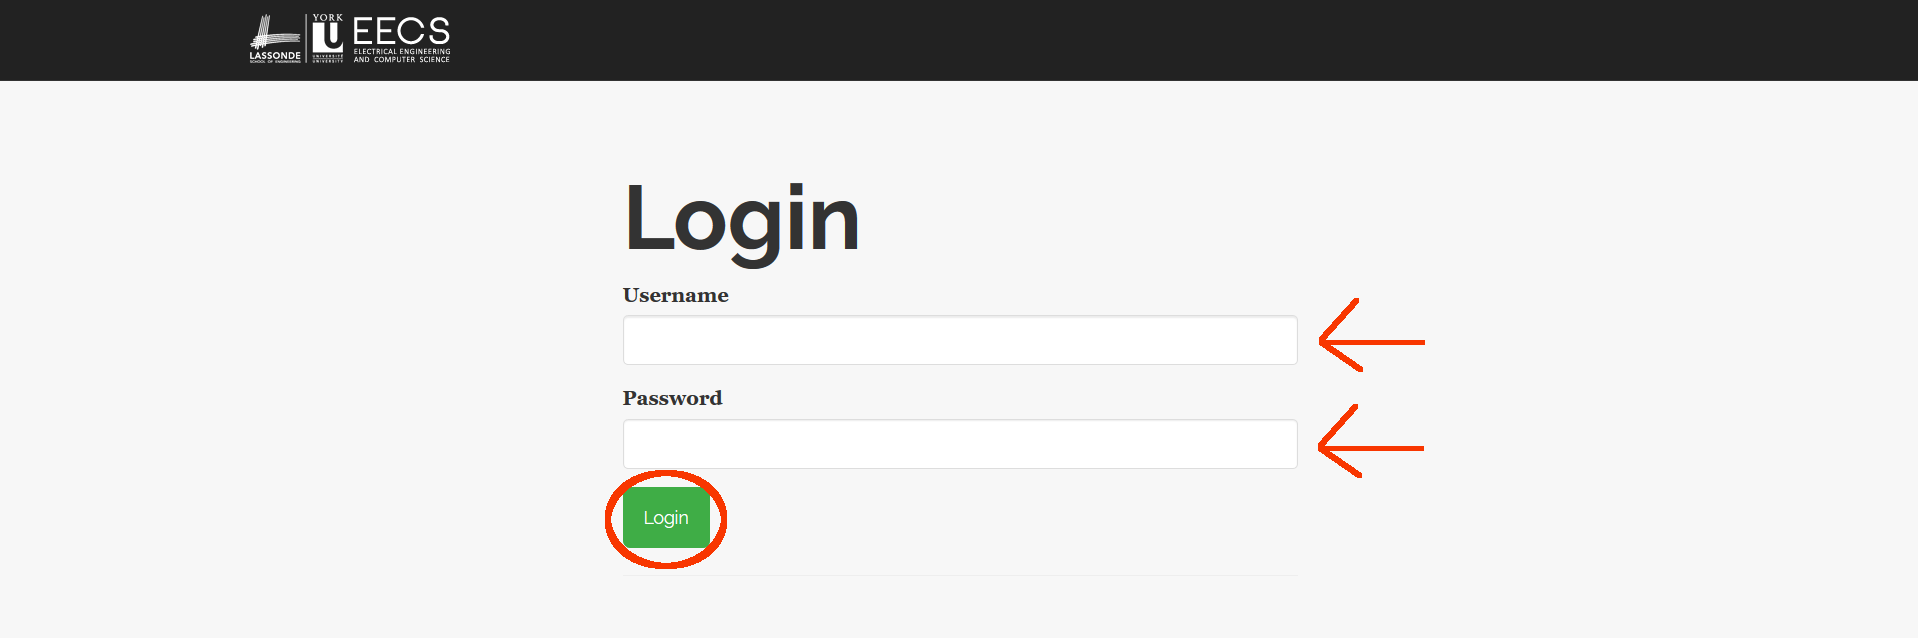
\includegraphics[width=.99\textwidth]{images/login.png}
\end{center}
\caption{Login Page}
\label{fig:login}
\end{figure}
\noindent \textbf{Note:} If the credentials you have provided are invalid you will be greeted with an error message.

\clearpage

\section{Selecting a Role}
To access the professor portal you must be signed in and select the professor role. The subsections below describe the methods for selecting the professor role.

\subsection{Role Selection Page}
From the role selection page click on the 'Continue as Professor" button to be redirected to the professor portal.

\begin{figure}[!htb]
\begin{center}
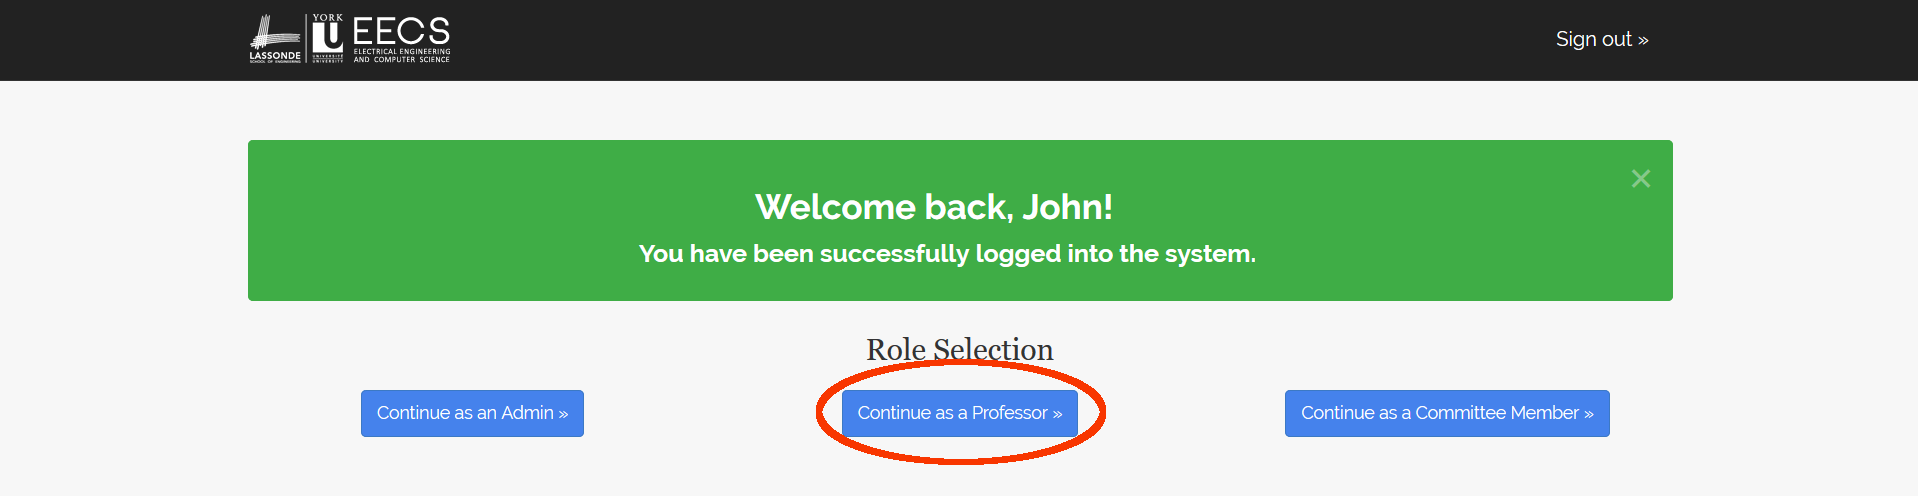
\includegraphics[width=.99\textwidth]{images/role-selection.png}
\end{center}
\caption{Role Selection Page}
\label{fig:role_selection1}
\end{figure}

\noindent \textbf{Note:} To access the administrator/committee/professor portal you must be granted access from an administrator.

\subsection{Navigation Bar}
If you have selected another role and wish to switch roles you will be presented with an option on the navigation bar. Click on the dropdown menu that displays your current role and click on your desired role.
\begin{figure}[!htb]
\begin{center}

\includegraphics[width=.99\textwidth]{images/role-selection2.png}
\end{center}
\caption{Switch Roles}
\label{fig:role_selection2}
\end{figure}

\noindent \textbf{Note:} To access the admin/committee/professor portal you must be granted the respective permissions from an admin.

\clearpage

Once you have selected the professor role you will should see a page similar to the one below

\begin{figure}[!htb]
\begin{center}
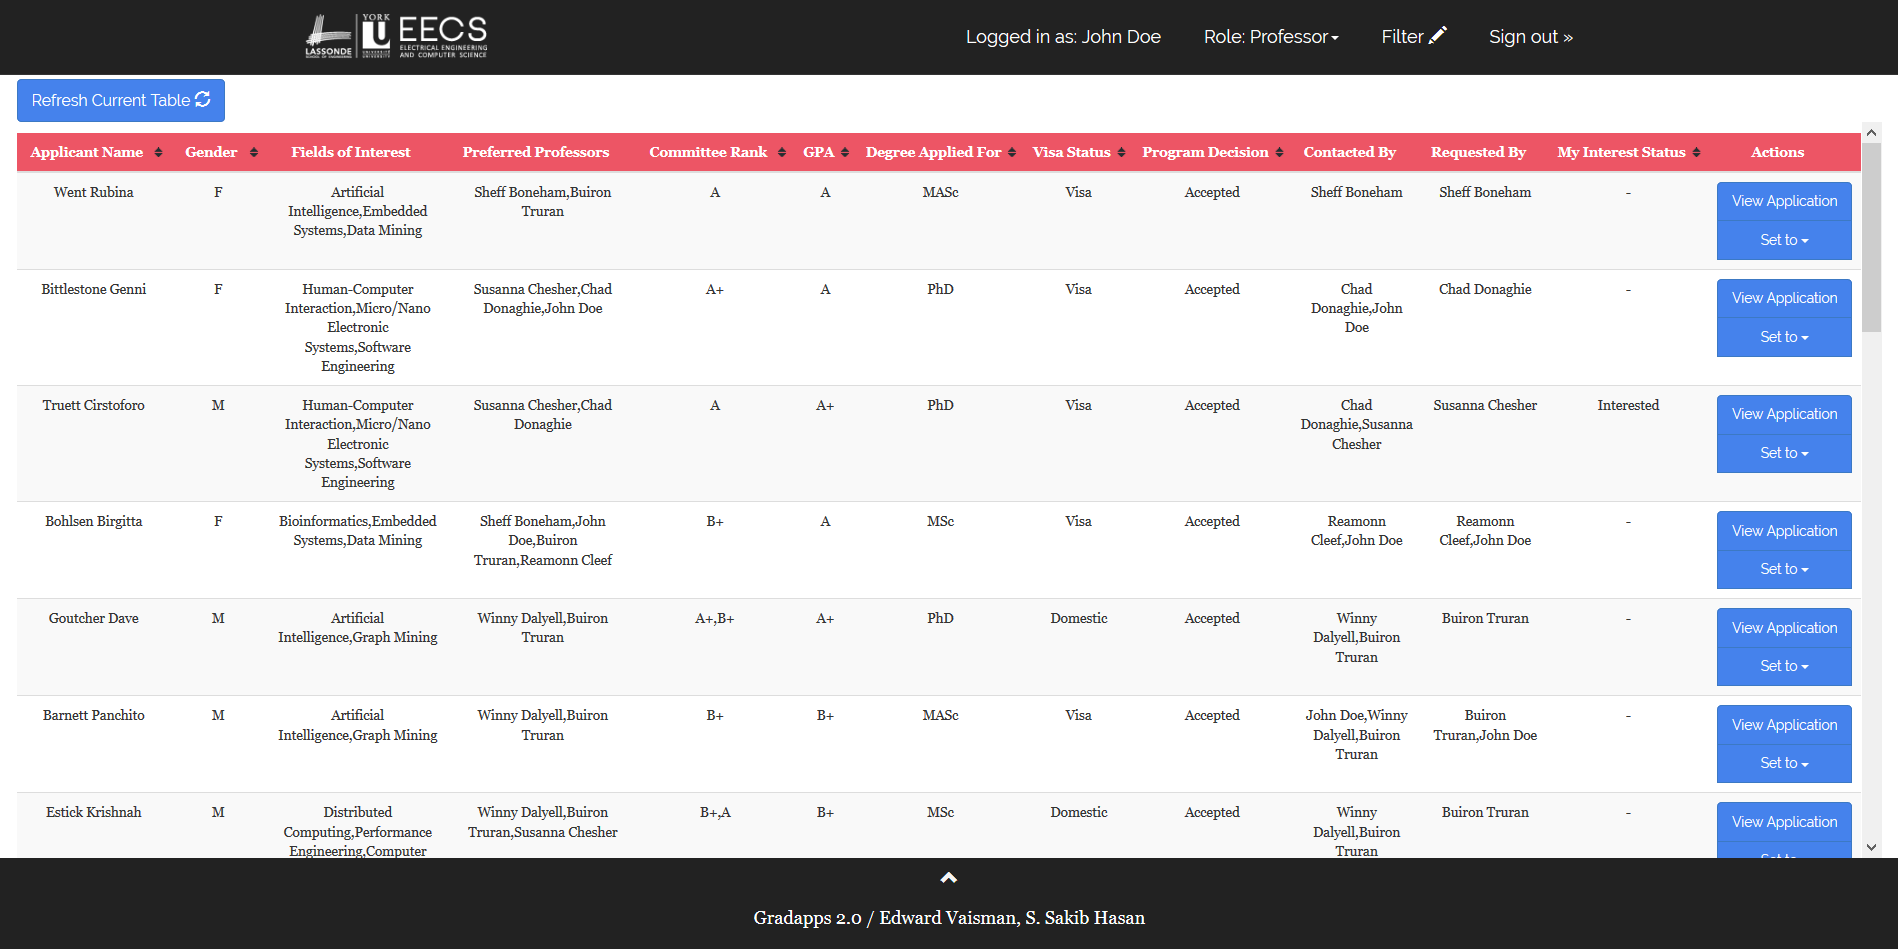
\includegraphics[width=.99\textwidth]{images/professor.png}
\end{center}
\caption{Professor Page}
\label{fig:professor}
\end{figure}

\clearpage
\section{Professor Portal}
\subsection{Filtering the Table}
Once you have been given access to the professor portal you will be granted the ability to see all the students who have applied. To help find applications that are relevant to you, simply filter the table using the steps below.

\subsubsection{Opening The Modal}
First open the modal. To do so click on the 'Filter" button on the navigation bar.

\begin{figure}[!htb]
\begin{center}
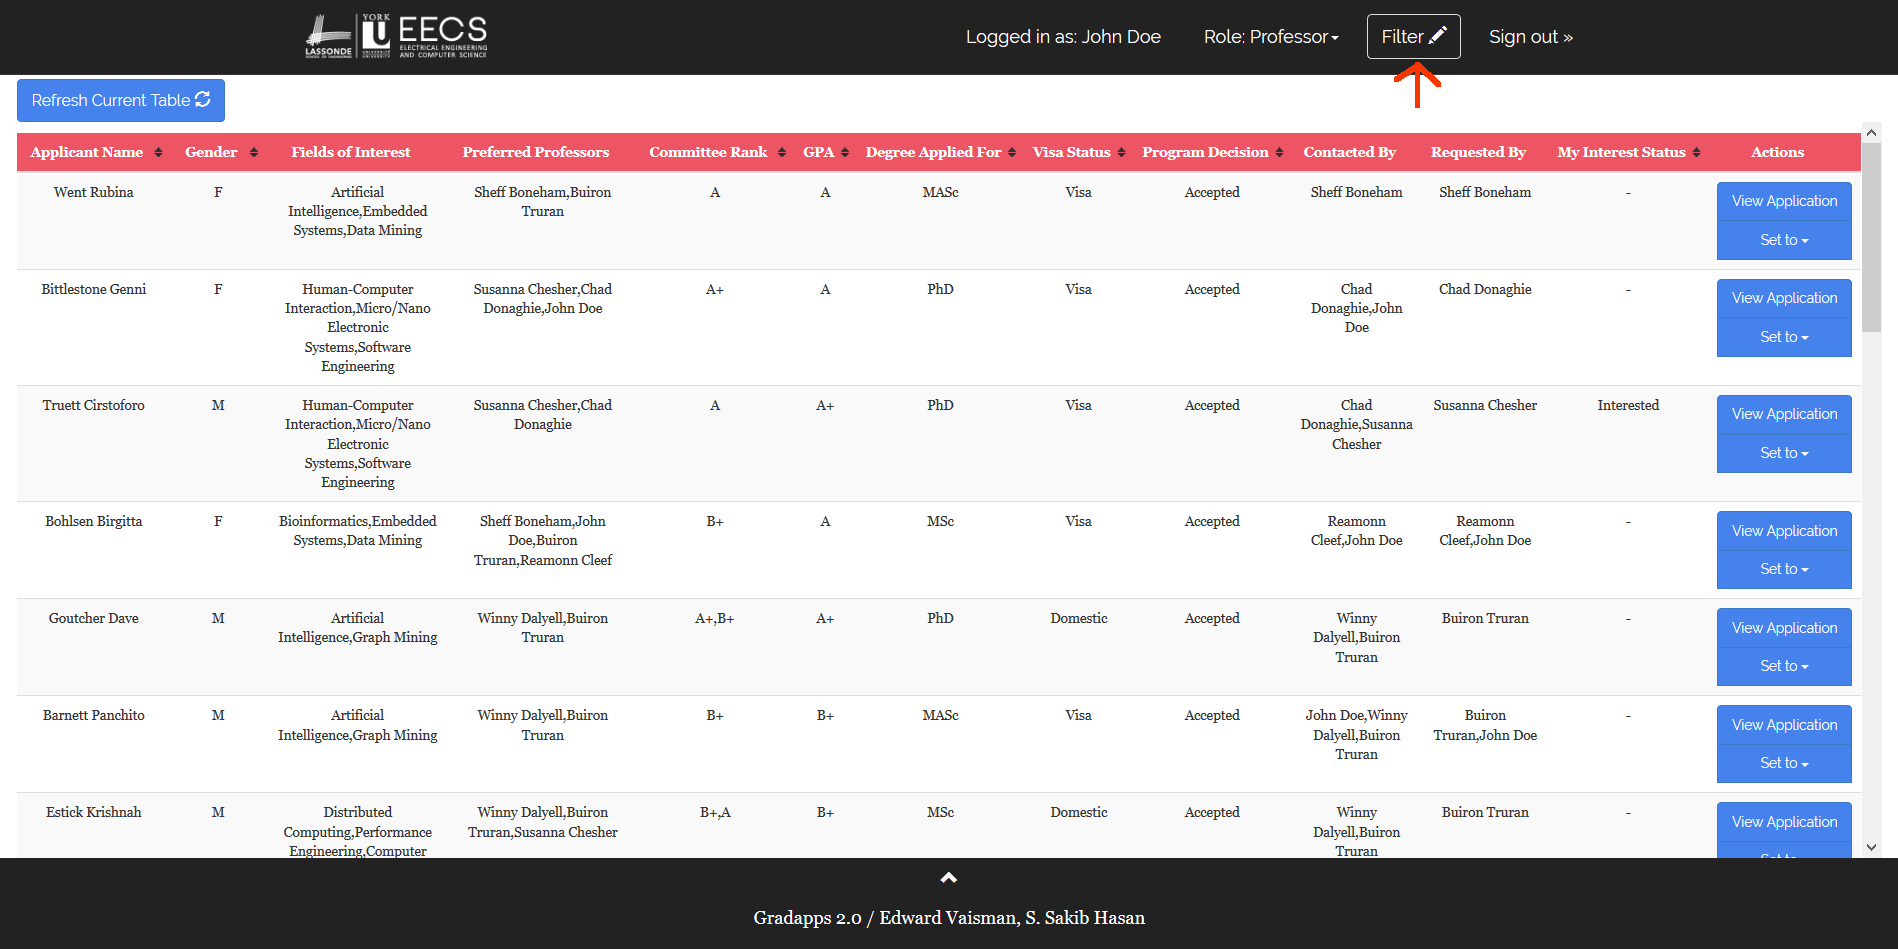
\includegraphics[width=.99\textwidth]{images/open_modal.png}
\end{center}
\caption{Open Modal}
\label{fig:open_modal}
\end{figure}

\begin{figure}[!htb]
\begin{center}
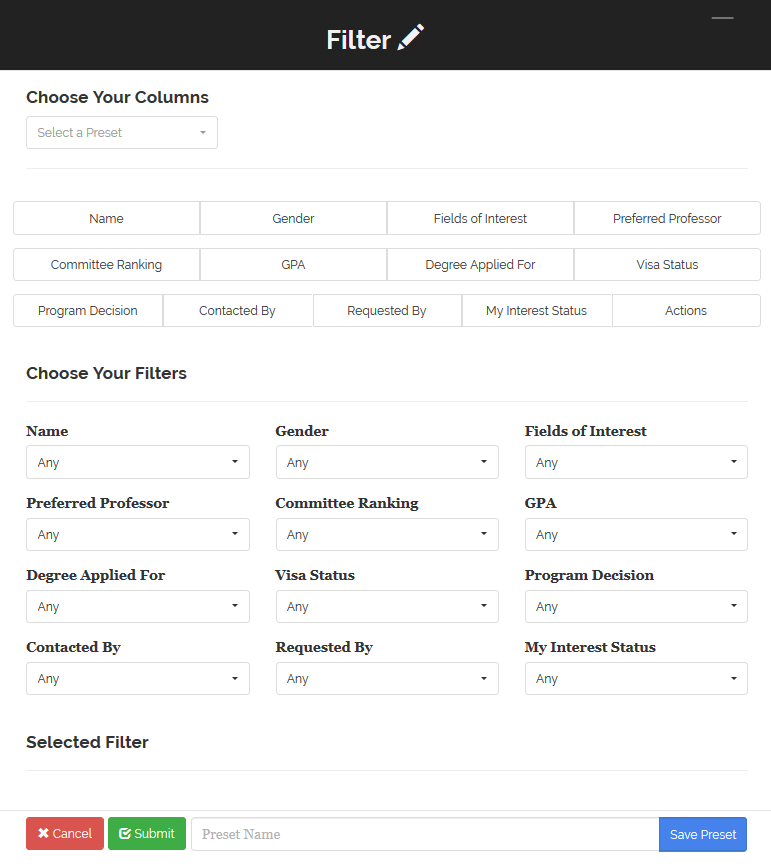
\includegraphics[width=.99\textwidth]{images/filter_view.png}
\end{center}
\caption{Filter View}
\label{fig:filter_view}
\end{figure}

\clearpage
\begin{figure}[!htb]
\subsubsection{Choose Your Columns}
The first step to filtering is to choose the columns you which to be displayed on the table. To do so just click on the button indicating which column you wish to see. Once clicked the button will display the order the columns will be displayed in as well.
\begin{center}
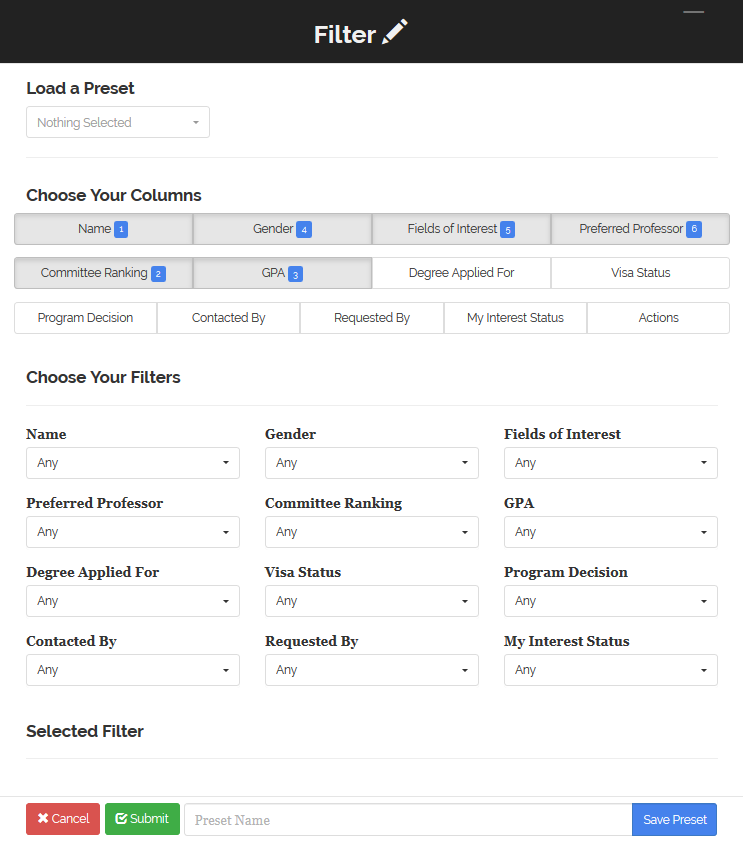
\includegraphics[width=.99\textwidth]{images/choose_columns.png}
\end{center}
\caption{Choose Your Columns}
\label{fig:choose_columns}
\end{figure}

\clearpage

\begin{figure}[!htb]
\subsubsection{Choose Your Filters}
The second step to filtering is to choose how you would like to filter the table. Begin by clicking on the drop down of the attribute you which to filter by and select an option from a list of generated options. You can use the search bar to help look for certain options.
\begin{center}
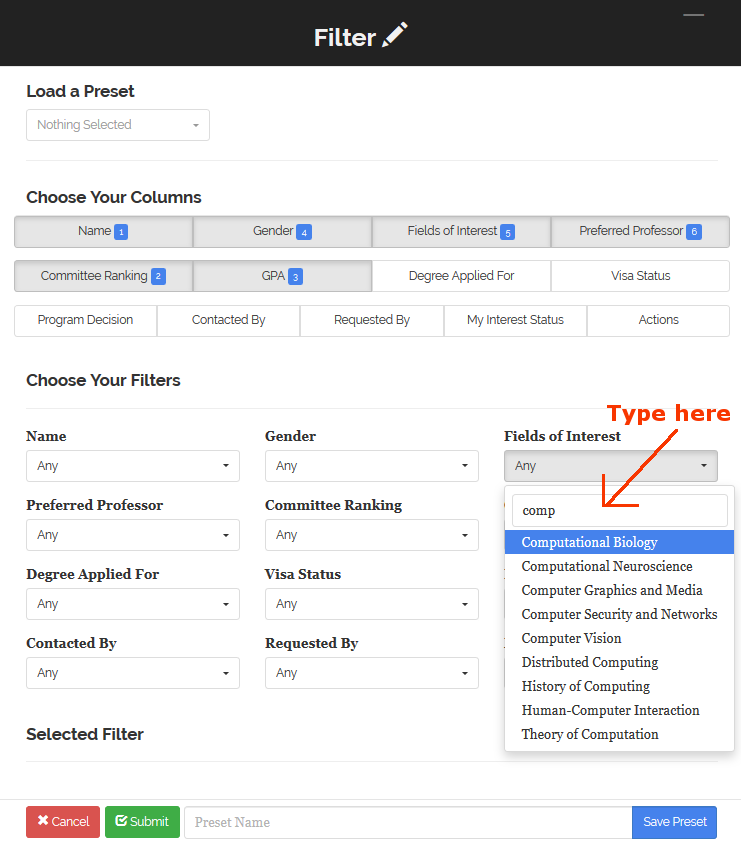
\includegraphics[width=.99\textwidth]{images/choose_filters.png}
\end{center}
\caption{Choose Your Filters}
\label{fig:choose_filters}
\end{figure}

\clearpage 
\begin{figure}[!htb]
\subsubsection{Submitting a Filter}
Once you have chosen your columns and filter attributes all that is left is to confirm your filter. Do so by checking the selected filter section for the filter attributes you have selected. Once that is done click submit
\begin{center}
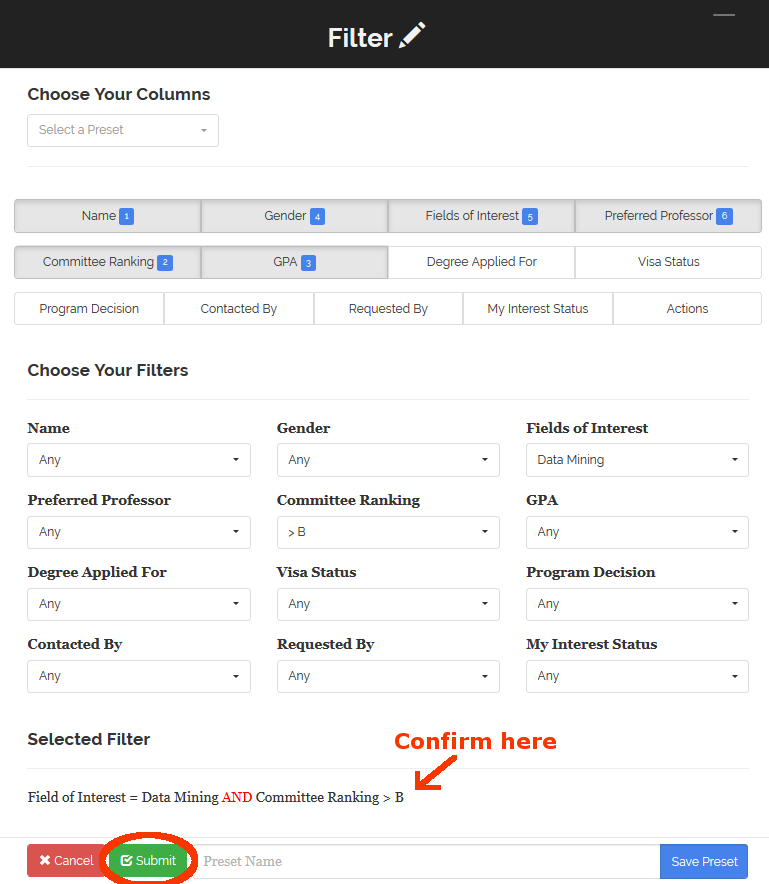
\includegraphics[width=.99\textwidth]{images/submit_filter.png}
\end{center}
\caption{Submit Filter}
\label{fig:submit_filter}
\end{figure}

\clearpage
Once you have submitted a filter you will be provided with a new table based on the filter provided. Attributes that satisfy your filter will be highlighted.
\begin{figure}[!htb]
\begin{center}
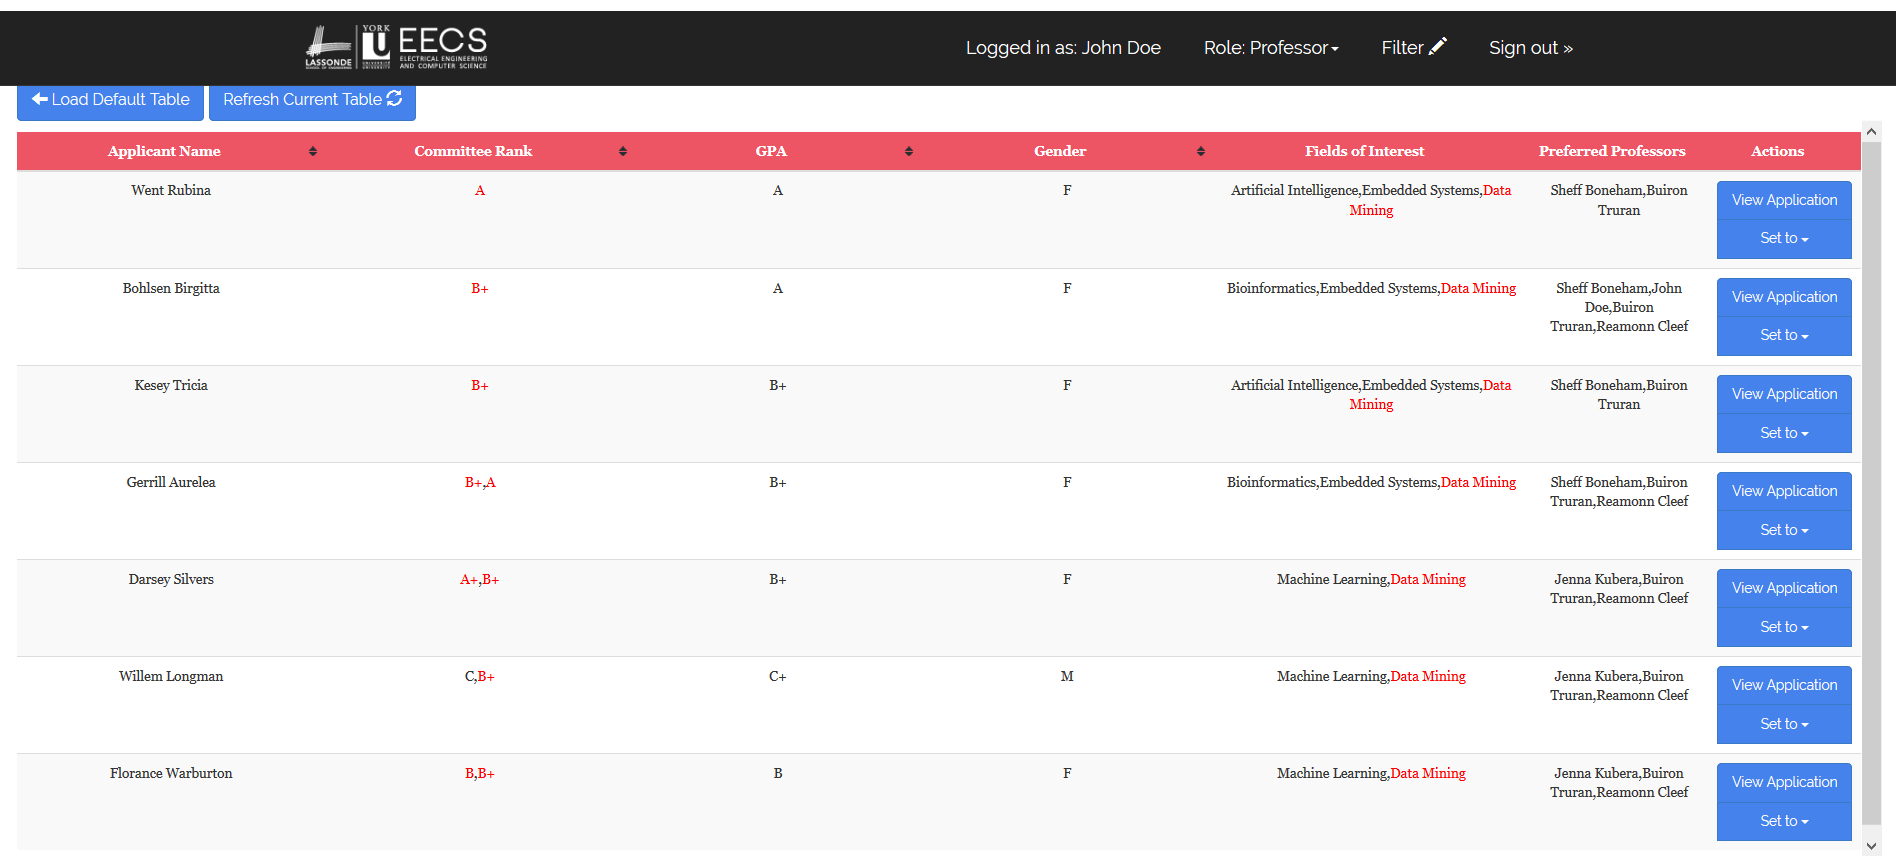
\includegraphics[width=.99\textwidth]{images/filtered_table.png}
\end{center}
\caption{Filtered Table}
\label{fig:filtered_table}
\end{figure}

\clearpage 
\subsubsection{Saving a Filter}
To save a filter give a name for the preset and click on 'Save Preset"
\subsubsection{Loading a Filter}
\subsection{Sorting the Table}
\subsubsection{Name}
\subsubsection{Gender}
\subsubsection{Committee Rank}
\subsubsection{GPA}
\subsubsection{Degree Applied For}
\subsubsection{Visa Status}
\subsubsection{Program Decision}
\subsubsection{Interest Status}
\subsection{Viewing an Application}
\subsection{Setting Application Attributes}
\subsubsection{Contacted By}
\subsubsection{Requested By}
\subsubsection{My Interest Status}


\end{document}
